\documentclass[12pt,a4paper]{article}
\usepackage{graphicx}
% uncomment according to your operating system:
% ------------------------------------------------
\usepackage[latin1]{inputenc}    %% european characters can be used (Windows, old Linux)
%\usepackage[utf8]{inputenc}     %% european characters can be used (Linux)
%\usepackage[applemac]{inputenc} %% european characters can be used (Mac OS)
% ------------------------------------------------
\usepackage{authblk}
\usepackage[superscript]{cite}
\usepackage[document]{ragged2e}
\usepackage[T1]{fontenc}   %% get hyphenation and accented letters right
\usepackage{mathptmx}      %% use fitting times fonts also in formulas
% do not change these lines:
\pagestyle{empty}                %% no page numbers!
\usepackage[left=35mm, right=35mm, top=15mm, bottom=20mm, noheadfoot]{geometry}
%% please don't change geometry settings!

\usepackage{fullpage}
\usepackage{amsfonts}
\usepackage{graphicx}
\usepackage{float}
\usepackage{amsmath}
\usepackage{chemfig}
\usepackage{indentfirst}
\usepackage{longtable}
\usepackage{array}
\usepackage{cellspace}
\usepackage{palatino}
%\usepackage{breqn}
\usepackage{amssymb}
\usepackage{verbatim}
\usepackage[colorlinks=true,citecolor=blue,linkcolor=blue]{hyperref}
\usepackage{siunitx}
\usepackage{xr}
\usepackage{enumitem}

\usepackage{setspace}
\usepackage{soul}

\singlespacing

% italicized boldface for math (e.g. vectors)
\newcommand{\bfv}[1]{{\mbox{\boldmath{$#1$}}}}
% non-italicized boldface for math (e.g. matrices)
\newcommand{\bfm}[1]{{\bf #1}}          

%\newcommand{\bfm}[1]{{\mbox{\boldmath{$#1$}}}}
%\newcommand{\bfm}[1]{{\bf #1}}
\newcommand{\expect}[1]{\left \langle #1 \right \rangle} % <.> for denoting expectations over realizations of an experiment or thermal averages

\newcommand{\var}[1]{{\mathrm var}{(#1)}}
\newcommand{\x}{\bfv{x}}
\newcommand{\y}{\bfv{y}}
\newcommand{\f}{\bfv{f}}
\newcommand{\C}{\bfm{C}}

\newcommand{\hatf}{\hat{f}}

\newcommand{\bTheta}{\bfm{\Theta}}
\newcommand{\btheta}{\bfm{\theta}}
\newcommand{\bhatf}{\bfm{\hat{f}}}
\newcommand{\Cov}[1] {\mathrm{cov}\left( #1 \right)}
\newcommand{\T}{\mathrm{T}}                                % T used in matrix transpose

\newcommand\blfootnote[1]{%
	\begingroup
	\renewcommand\thefootnote{}\footnote{#1}%
	\addtocounter{footnote}{-1}%
	\endgroup
}

\usepackage{natbib}
\setlength{\bibsep}{0.0pt}

%\usepackage[style=authoryear-icomp,maxbibnames=9,maxcitenames=1,uniquelist=false,
%backend=biber]{biblatex}
\bibliographystyle{unsrt}

% begin the document
\begin{document}
	\thispagestyle{empty}
	%make title bold and 14 pt font (Latex default is non-bold, 16 pt)
	\title{\Large \textbf{Humboldt Research Fellowship}}
	\author[1]{\large {\underline{Richard Messerly}}}%%[12 pt regular, presenting speaker underlined]
	
	\affil[1]{\textit{Thermodynamics Research Center (TRC), National Institute of Standards and Technology (NIST),
			Boulder, Colorado, 80305, USA}}
	
	\date{} % <--- leave date empty
%	\maketitle\thispagestyle{empty} %% <-- you need this for the first page
%	\begin{center}
%		\title{\textbf{ABSTRACT}}\centering{}
%	\end{center}
	\justify

%\section*{Description of proposal guidelines on Humboldt website}
%
%The current state of research should first be briefly described and supported by approximately five revelant publications from the research area (one page max).
%
%The outline should focus on a clear description of the questions you intend to address in your research, their originality and significance for the advancement of the research field (approx. two pages).
%
%Furthermore, the academic methods to be used to achieve these goals should be clearly described and referenced, if appropriate (approx. two pages).
%
%The research outline should comprise approximately five pages in total (including references). Should you significantly exceed this length, you may be asked to cut it down to approximately five pages.
%
%For the purposes of evaluation it must be clearly demonstrated that you yourself have drawn up the main contents independently and agreed them beforehand with your host. Any contents contributed by the host institute must be attributed accordingly.

\section*{Advancing the hybrid data set approach towards reliable mixture properties: Going beyond the traditional Lennard-Jones potential}

%Title ideas 1) Developing self-consistent equations of state and force fields 2) Advancing the hybrid data set approach: Going beyond the traditional Lennard-Jones potential 3) High accuracy force fields for prediction of mixture properties 

The understanding of natural mechanisms and design of efficient and reliable technical processes rests on the accurate knowledge of thermophysical properties of fluids over a wide range of temperatures and pressures. Fundamental equations of state (FEOS), such as those based on the Helmholtz energy ($A$), are a powerful approach for consistently representing the pressure, density, temperature $(P\rho T)$ behavior together with caloric properties, such as internal energy $(U)$ and isochoric/isobaric heat capacities $(c_{\rm v}$ and $c_{\rm p}$, respectively) of pure species and mixtures. The National Institute of Standards and Technology (NIST) is the global leader in FEOS development. During my postdoctoral associateship at NIST, I have been fortunate to collaborate with the developers of the NIST FEOS, Reference Fluid Properties (REFPROP \cite{LEMMON-RP91}). 

%In addition, I attended the 19th and 20th Symposium on Thermophysical Properties, where sessions are dedicated to advances in FEOS development.  On a triennial basis, NIST organizes The Symposium on Thermophysical Properties.

In general, FEOS separate the Helmholtz energy into an ideal gas $(A^{\rm ig})$ and a residual $(A^{\rm r})$ contribution. As $A^{\rm ig}$ is typically obtained using first principles (\textit{ab initio}) calculations, the primary focus of FEOS development is modeling $A^{\rm r}$. State-of-the-art FEOS, such as those collected in REFPROP, utilize a semi-empirical model for $A^{\rm r}$ with between 50 and 100 non-linear fitting parameters. The number of fitting parameters and, thence, the FEOS accuracy is determined by the quality, quantity, and diversity of experimental data. When an FEOS correlation is reliable over the entire fluid region of technological interest, it is considered to be of ``technical accuracy.'' 

Since most fluids are mixtures of several molecular species, reliable estimates of mixture properties are essential. The development of mixture FEOS is, thus, a key endeavor at NIST and several sessions were dedicated to this topic at the 20$^{\rm th}$ Symposium on Thermophysical Properties organized by NIST in 2018. The primary challenge is that experimental mixture data are of questionable quality and are relatively scarce. This scarcity is insurmountable as the phase space dimensionality increases with the number of species due to the additional composition variable(s). The data shortage is especially troubling since mixture FEOS require additional fitting parameters for $A^{\rm r}$. An equally important issue is that any deficiencies in the pure species FEOS propagate when predicting mixture properties. Therefore, the ability to develop ``technical accuracy'' mixture FEOS necessitates ``technical accuracy'' pure species FEOS. For this reason, the discussion that follows focuses on pure species. 

%while experimental mixture data are scarce (due to the additional composition variable) and of questionable quality.

Unfortunately, most compounds do not have sufficient \textit{reliable} experimental data for a diverse set of thermodynamic properties covering a wide range of $P \rho T$ conditions to develop a ``technical accuracy'' FEOS. Consequently, REFPROP covers less than 100 compounds with ``technical accuracy.'' Due to the large amount of fitting parameters, FEOS predictions can result in substantial errors when extrapolated to higher temperatures and pressures than those of the training data. Improvement in an FEOS necessitates additional data at these extreme temperatures and pressures. The lack of experimental data under these conditions is attributed to the inherent safety, cost, and complexity of such experiments (e.g., chemical instability above the thermal decomposition temperature).

By contrast, molecular simulation (i.e. Monte Carlo, MC, and molecular dynamics, MD) methods do not suffer from any of these limitations. For this reason, the host, Vrabec, and coworkers proposed the use of ``hybrid data sets'' consisting of both available experimental data and molecular simulation results at extreme temperatures and pressures  \cite{Rutkai2013}. Together with collaborators, Vrabec has  demonstrated for several compounds that hybrid data sets extend the range of applicability for the FEOS \cite{Thol2016_siloxane_first,Thol2016_siloxane,Thol2017,Rutkai2013,Thol2015}. 

The simulation values that are included in hybrid data sets are derivatives of the residual Helmholtz energy with respect to inverse temperature and/or density
\begin{equation} \label{Residual Derivatives}
A_{xy}^{\rm r} R_gT \equiv (1/T)^x\rho^y \frac{\partial^{x+y}A^{\rm r}}{\partial(1/T)^x \partial \rho^y}
\end{equation}
where $R_g$ is the gas constant. We would like to emphasize the advantage of using $A_{xy}^{\rm r}$ for developing FEOS, as this choice eliminates redundant information found in traditional macroscopic properties \cite{Thol2016_LJ,Thol_LJTS,Rutkai2017,Lustig2015,Rutkai2013,Rutkai2015}. Furthermore, experimental data are typically measured for properties that relate only to first and second derivatives, whereas, in principle, molecular simulation provides an avenue for estimating higher order derivatives, which could be invaluable when fitting FEOS. 

%The infrastructure is already in place to implement the hybrid data set approach at the host institute, Technische Universitat Berlin. Specifically, Vrabec's group have developed \textit{ms2} \cite{ms2}, a highly optimized and parallelized code written in Fortran 90 that is capable of performing both MC and MD simulations. More importantly, \textit{ms2} is the only open-source simulation package that computes $A_{xy}^{\rm r}$ for various values of $x$ and $y$. In addition, Vrabec's group has already automated the entire process of simulating the necessary $P \rho T$ state space and processing the $A_{xy}^{\rm r}$ results with minimal human interaction. With access to tens of thousands of cores on a supercomputer, Vrabec's group is capable of generating all the required molecular simulation results for a given force field in just a few hours.
 
%has already been automated by Vrabec's group with minimal human interaction. 
 
%The inclusion of $A_{xy}^{\rm r}$ simulation results greatly improved the extrapolation of the FEOS to extreme temperatures and pressures.
%Recently,  successfully applied this ``hybrid data set'' approach to dramatically extend the FEOS' range of applicability for several compounds \cite{Rutkai2013,Thol2016_siloxane_first,Thol2016_siloxane,Thol2017,Thol2015}.

The primary limitation of the hybrid data set approach is that most force fields are not ``transferable'' over a wide range of $P \rho T$ conditions. This deficiency causes the force field to be inconsistent with the FEOS. For example, in a recent study \cite{Messerly2018_2}, we demonstrated poor transferability to high pressures of the popular Mie $n$-6 potential for normal and branched alkanes. Specifically, as the Mie $n$-6 potential requires $n \ge 14$ to accurately predict vapor-liquid equilibrium (VLE) properties, it is overly-repulsive at short distances, resulting in significant deviations at high densities/pressures. Therefore, Mie $n$-6 force fields (of which the traditional Lennard-Jones 12-6 is a subclass) are ill-suited for the hybrid data set approach.

The question that this study will address is, \ul{can a pairwise additive force field have the same ``technical accuracy'' as the FEOS?} As thermodynamic properties are extremely sensitive to  intermolecular interactions, \textbf{we propose that more flexible and physically realistic non-bonded potential functions be considered when developing FEOS.} For example, \textit{ab initio} based two-body potentials typically utilize more than ten fitting parameters (see Equation 6 of Reference \citenum{Hellmann2017}). 

% because of the high information content in \textit{ab initio} energy calculations performed at different interatomic distances,

%because of the high information content in \textit{ab initio} energy calculations performed at different interatomic distances

% we focus primarily on developing extremely flexible intermolecular potential functions.

%The poor extrapolation was due to $n > 12$ leading to overly repulsive forces at high densities.

% this is that the optimal value of $n$ to reproduce saturated vapor and liquid properties is typically greater than 12 (e.g. the Potoff 16-6 potential). Unfortunately, $n \gg 12$ is not theoretically justified and leads to an overly repulsive potential at high densities.

%To improve the performance of this so-called ``hybrid data set'' approach, it is imperative that the force field be transferable over different $P \rho T$ conditions. Therefore, we propose that more theoretical and flexible potential models be considered for developing FEOS. Specifically, we propose the development of extended Lennard-Jones (ex-LJ) force fields to improve the fundamental equations of state at high pressures.

%In a previous study, we demonstrated the poor transferability to high pressures of the popular united-atom Mie $n$-6 potential (of which the traditional Lennard-Jones 12-6 is a subclass). 

%To improve this method, we propose that more theoretical and flexible non-bonded potential functions be considered for developing FEOS. For example, two body potentials developed from \textit{ab initio} values typically utilize five to ten fitting parameters because of the high information content in \textit{ab initio} calculations at different intermolecular distances.

For nearly half a century the Lennard-Jones (LJ) 12-6 potential has inundated the molecular simulation literature (the popular choice of $n=12$ has no theoretical basis and is a historical artifact based primarily on computational reasons that are no longer significant). Only in the past decade has the Mie $n$-6 potential received considerable attention. However, due to inadequacies in the Mie $n$-6 potential at high pressures, \textbf{we propose the development of extended Lennard-Jones (ex-LJ) force fields for the hybrid data set approach.} 

The general expression for the extended Lennard-Jones non-bonded potential is
\begin{equation} \label{ex-LJ general}
u_{\rm nb, ex\text{-}LJ}(\C) = \sum_{m = 6, 8 ...} C_m r^{-m} 
\end{equation} 
where $m$ are integer (typically even) values and the parameter set, $\C$, consists of the $C_m$ coefficients corresponding to the $r^{-m}$ terms. Note that the traditional Lennard-Jones 12-6 potential is obtained if $C_{12} = 4\epsilon\sigma^{12}$ and $C_6=-4\epsilon\sigma^{6}$ (where $\sigma$ and $\epsilon$ are the Lennard-Jones size and energy parameters, respectively), while all other $C_m$ values are zero. The attractive terms (negative $C_m$) are derived rigorously from London dispersion forces \cite{Stone2013}. By contrast, the repulsive terms (positive $C_m$) are strictly empirical and, if necessary, can be replaced by more physical functions (e.g., $\exp(-r)$ \cite{Hellmann2017,Przybytek2017}). 

%Typically, \textit{ab initio} based two-body potentials only include $r^{-6}$, $r^{-8}$, and $r^{-10}$ terms, as the contributions from higher order terms are negligible for .

%can be derived rigorously from attractive London dispersion interactions \cite{Stone2013}. By contrast, the repulsive terms (positive $C_m$, typically $m > 10$) are strictly empirical.

The ex-LJ potential is more flexible than the two-parameter ($\epsilon$ and $\sigma$) LJ 12-6, and more theoretically justified than the three-parameter Mie $n$-6, particularly when $n \gg 12$. However, it has not been tested as extensively as the LJ 12-6, Mie $n$-6, and exponential-6 potentials. By demonstrating significant improvement at high pressures, \textbf{the potential impact of this research would be to initiate a paradigm shift in non-bonded potentials.}

The question remains, when a sufficient number of non-zero terms is included in Equation \ref{ex-LJ general}, \ul{can an ex-LJ force field fit higher order derivatives of the Helmholtz energy over the entire fluid region of technological interest?} The development of ``technical accuracy'' ex-LJ force fields will allow for the prediction of other properties not available from the FEOS, such as transport properties (e.g., self-diffusivity, shear viscosity) and structural/non-equilibrium phenomena, as well as various mixture properties.

%Traditionally, there are only two to four non-zero $C_m$ values, e.g., 16-6, 12-8-6, 14-12-8-6. The primary reasons for this are to simplify the parameterization and to avoid over-fitting if the data are insufficient to characterize more parameters. In principle, however, any number of $C_m$ terms could be non-zero. 

%As the ex-LJ has received relatively little attention in the literature, some additional questions naturally arise. For example, since most \textit{ab initio} based two-body potentials utilize $r^{-6}$, $r^{-8}$, and $r^{-10}$ terms for attractive interactions, \ul{should the $C_6$, $C_8$, and $C_{10}$ coefficients necessarily be negative?} Similarly, \underline{how many non-zero terms in Equation \ref{ex-LJ general}}\ul{ should be included such that the model is sufficiently flexible but not over-fit?} \ul{Which terms provide the greatest improvement in the force field?} \ul{Which combining rules (e.g., Lorentz-Berthelot) should be used for cross interactions?} 

As the ex-LJ has received relatively little attention in the literature, some additional questions naturally arise. For example, since most \textit{ab initio} based two-body potentials utilize $r^{-6}$, $r^{-8}$, and $r^{-10}$ terms for attractive interactions, should the $C_6$, $C_8$, and $C_{10}$ coefficients necessarily be negative? How many non-zero terms in Equation \ref{ex-LJ general} should be included such that the model is sufficiently flexible but not over-fit? Similarly, which terms provide the greatest improvement in the force field? Which combining rules (e.g., Lorentz-Berthelot) should be used for cross interactions?

Combining rules reduce the number of force field parameters that are optimized simultaneously for compounds with multiple interaction site types. More importantly, combining rules are essential for performing simulations of mixtures, which is a key motivation for developing ``technical accuracy'' force fields for pure species. While numerous combining rules are proposed in the literature for the LJ 12-6 parameters \cite{Schnabel2007}, combining rules for $C_m$ are less straightforward and will likely require innovative formulations.

%As the ex-LJ has received relatively little attention in the literature, some additional questions naturally arise. For example, \underline{which combining rules (e.g., Lorentz-Berthelot) should be used for cross interactions?} Combining rules simplify force field parameterization for compounds with multiple interaction site types. More importantly, combining rules are essential for performing simulations of mixtures, which is a key motivation for developing ``technical accuracy'' force fields for pure species. Although numerous combining rules are proposed in the literature for the Lennard-Jones parameters (cf., Reference \citenum{Schnabel2007}), combining rules for $C_m$ are less straightforward and will likely require innovative formulations.

%Since the $r^{-6}$, $r^{-8}$, and $r^{-10}$ terms can be derived from dispersive interactions, should their $C_m$ coefficients necessarily be negative. 
%
%Which $C_m$ coefficients should be negative? The $r^{-6}$, $r^{-8}$, and $r^{-10}$ terms can be derived from dispersive interactions and, therefore, $C_6$, $C_8$, and $C_{10}$ should be negative from a theoretical standpoint. 

% suggest that the attractive interactions are adequately represented 
%Most \textit{ab initio} based two-body potentials $C_6$, $C_8$
%Due to the theoretical basis of the $r^{-6}$, $r^{-8}$, and $r^{-10}$ terms, should the $C_6$, $C_8$, and $C_{10}$ coefficients necessarily be negative?

%Since most \textit{ab initio} based two-body potentials utilize $r^{-6}$, $r^{-8}$, and $r^{-10}$ terms for attractive interactions, should the $C_6$, $C_8$, and $C_{10}$ coefficients necessarily be negative? Similarly, how many non-zero terms in Equation \ref{ex-LJ general} should be included such that the model is sufficiently flexible but not over-fit? Which terms provide the greatest improvement in the force field? 

%However, it is unclear how well a 12-10-8-6 potential would perform if only the $C_{12}$ coefficient is positive. Therefore, from an empirical standpoint, it is possible to allow all coefficients to be either positive or negative.

%Without over-fitting, how many terms are required?

%Due to the additional model parameters of the ex-LJ, the traditional approach of performing molecular simulation with each proposed parameter set $(\theta)$ is computationally infeasible when several $C_m$ terms are non-zero.

Although the ex-LJ was proposed over three decades ago \cite{Kalos1972}, the main reason for the lack of popularity is the additional complexity in parameterizing the ex-LJ potential when several $C_m$ terms are non-zero. This presents another essential question, \ul{what optimization method is best suited for parameterizing the ex-LJ potential?} The development of an optimization scheme will \textbf{allow future researchers to parameterize ``technical accuracy'' ex-LJ force fields.}

%While \textit{ab initio} calculations provide rigorous access to the non-bonded potential, 
%neglect three-body and higher-body interactions, they 

% 
%Developing an ex-LJ force field based on \textit{ab initio} values is feasible . Unfortunately, \textit{ab initio} based two-body potentials do not perform well in liquid and supercritical phases and are, therefore, ill-suited for developing ``technical accuracy'' force fields. Rigorously accounting for three-body and higher-body interactions with \textit{ab initio} methods is an arduous task. Instead, accurate prediction of condensed phase properties is often achieved by developing effective non-bonded parameters (which indirectly account for three-body and higher-body interactions). 

%, fitting an ex-LJ force field to \textit{ab initio} results i \textit{ab initio} based two-body potentials are opt

%Developing an \textit{ab initio} based ex-LJ potential is  
%Because of the high information content in \textit{ab initio} energy calculations performed at different interatomic distances, simultaneous optimization of several $C_m$ terms is feasible. Unfortunately, 
%\textit{ab initio} based two-body potentials do not perform well in liquid and supercritical phases and are, therefore, ill-suited for developing ``technical accuracy'' force fields. Although it is possible to account for three-body interactions with \textit{ab initio} methods, this is an arduous task, especially for multiple-site molecules. Instead, accurate prediction of condensed phase properties is often achieved by developing effective non-bonded parameters (which indirectly account for three-body and higher-body interactions).
%
%Simultaneous optimization of several non-zero $C_m$ terms with \textit{ab initio} energy calculations performed at different interatomic distances is feasible due to the high in

\textit{Ab initio} energy calculations performed at different intermolecular distances have high information content regarding the non-bonded interactions. Unfortunately, \textit{ab initio} based two-body potentials do not perform well in liquid and supercritical phases and are, therefore, ill-suited for developing ``technical accuracy'' force fields. Accounting for three-body interactions is an arduous task with \textit{ab initio} methods, especially for multiple-atom molecules, and provides only marginal improvement. Instead, accurate prediction of condensed phase properties is often achieved by developing effective non-bonded parameters (which indirectly account for three-body and higher-body interactions).

%Because of the high information content in , simultaneous optimization of several non-zero $C_m$ terms is feasible. Unfortunately, 
%\textit{ab initio} based two-body potentials do not perform well in liquid and supercritical phases and are, therefore, ill-suited for developing ``technical accuracy'' force fields. Although it is possible to account for three-body interactions with \textit{ab initio} methods, this is an arduous task, especially for multiple-site molecules. Instead, accurate prediction of condensed phase properties is often achieved by developing effective non-bonded parameters (which indirectly account for three-body and higher-body interactions).
%
% Accounting for three-body interactions with \textit{ab initio} methods is an arduous task, especially for multiple-atom molecules, with only marginal improvement.

% Instead, effective non-bonded potentials (which indirectly account for three-body and higher-body interactions) are parameterized empirically to macroscopic condensed phase properties. 

For example, previous hybrid data set studies optimized the non-bonded parameters to VLE data, e.g., saturated liquid density and saturated vapor pressure. However, it is unlikely that VLE properties alone can provide a unique set of parameters for a highly flexible potential, such as the ex-LJ with more than three non-zero $C_m$ terms. By contrast, derivatives of Helmholtz energy ($A_{xy}^{\rm r}$) provide high information content regarding the non-bonded potential. Unfortunately, reliable $A_{xy}^{\rm r}$ values require an accurate FEOS, which is not available \textit{a priori}. For this reason, \textbf{we propose a \textit{novel} iterative hybrid data set approach} (see Figure \ref{FlowChart}).

% where the number of non-zero $C_m$ terms increases at each iteration:

%\begin{enumerate}%[nolistsep]
%	\item Develop FEOS over $P \rho T$ range where reliable experimental data exist
%	\item Parameterize the ex-LJ force field with FEOS $A_{xy}^{\rm r}$ over $P \rho T$ region of applicability
%	\item Iterate: 
%	\begin{enumerate}[nolistsep]%[topsep=0pt,parsep=0pt]
%		\item Estimate $A_{xy}^{\rm r}$ for ex-LJ force field at extreme temperatures and pressures
%		\item Refit FEOS to the hybrid data set
%		\item Re-parameterize the ex-LJ force field using updated FEOS $A_{xy}^{\rm r}$
%	\end{enumerate}
%\end{enumerate}

\begin{figure}[htb!]
	\centering
	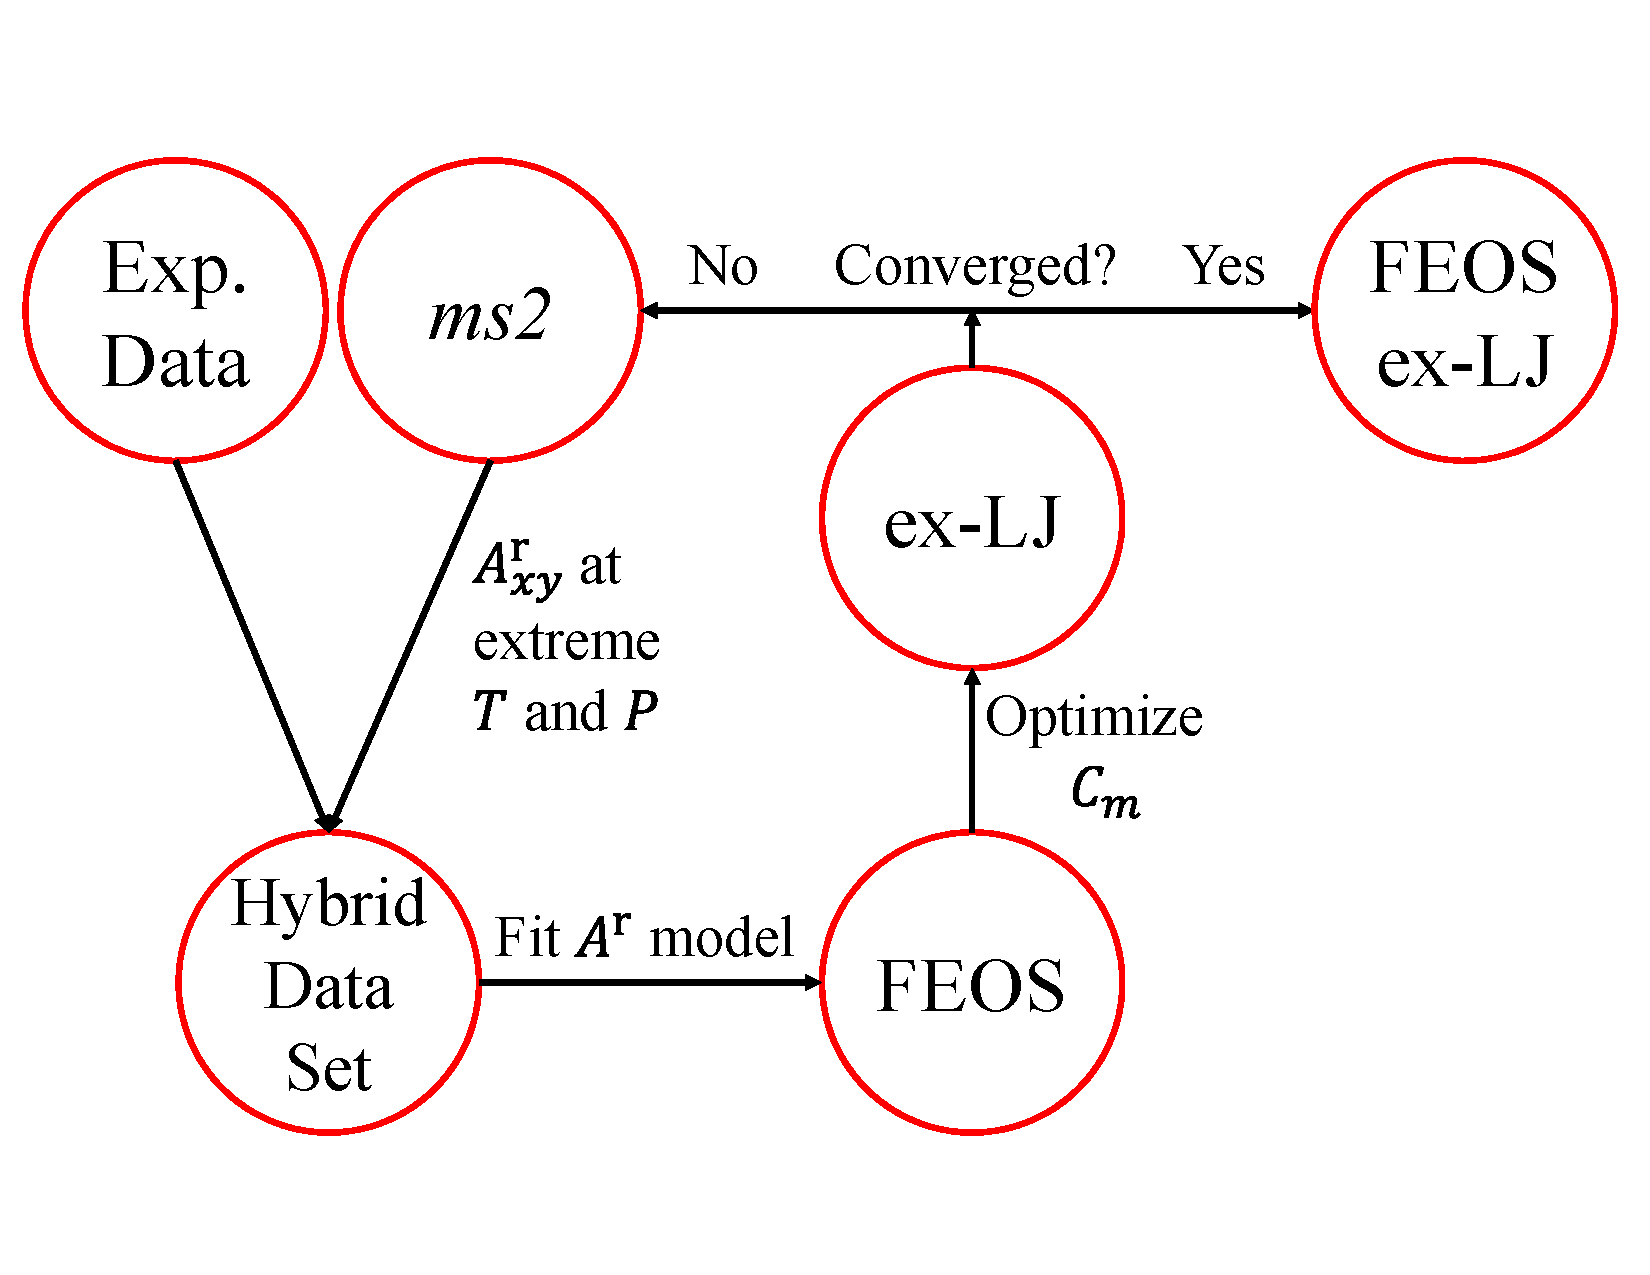
\includegraphics[width=4.0in]{FlowChart.pdf}
	\caption{Iterative hybrid data set approach for generating self-consistent FEOS and ex-LJ force field of ``technical accuracy.''}
	\label{FlowChart}
\end{figure}
%\vspace{-1cm}

% It remains to be seen how many state points  unique non-zero $C_m$ terms can be parameterized simultaneously.


%Basis functions are amenable to the extended Lennard-Jones potential. For example, the 

%Basis functions store the contributions from the $r^{-m}$ terms for the nonbonded energies and forces

%In previous hybrid data set studies, the LJ 12-6 parameters were optimized with VLE properties. The two reasons for this practice are the availability of VLE data and the difficulty of optimizing force field parameters. If several model parameters are included in Equation BLANK, the traditional approach of force field parameterization, namely, trial-and-error optimization is not computationally feasible. Furthermore, it is unlikely that VLE data alone can provide a unique set of parameters. By contrast, derivatives of Helmholtz energy provide high information content regarding the non-bonded potential. 

%The methodology proposed in this study is to:
%\begin{enumerate}
%	\item Develop a FEOS over the temperatures and pressures where reliable experimental data exist
%	\item Fit the ex-LJ parameters to FEOS derivative Helmholtz energy properties in range where FEOS is reliable
%	\item Perform molecular simulations at state points where experimental data are not available
%	\item Iterate:
%	\begin{enumerate}
%		\item Refit the FEOS to the hybrid data set
%		\item Re-optimize the force field parameters to match FEOS (using MBAR so that no additional molecular simulations are required)
%	\end{enumerate}
%\end{enumerate}

The iterative approach presented in Figure \ref{FlowChart} ensures that the Helmholtz energy derivative properties are internally consistent between the FEOS and the ex-LJ force field. The aim is to improve the extrapolation of the FEOS and the force field transferability. As the FEOS and ex-LJ force field become more self-consistent with each successive iteration, it is possible to increase the number of non-zero $C_m$ terms in Step 3), although this may necessitate including higher order derivatives (i.e., $A_{xy}^{\rm r}$ for $x+y>2)$.

The infrastructure is already in place to implement Steps 1) and 2) at the host institute, Technische Universit\"{a}t Berlin. Specifically, Vrabec's group developed \textit{ms}2 \cite{ms2}, a highly optimized and parallelized code that is capable of performing both MC and MD simulations. More importantly, \textit{ms}2 is the only open-source simulation package that computes $A_{xy}^{\rm r}$ for various values of $x$ and $y$. In addition, Vrabec's group has already automated the entire process of simulating the necessary $P \rho T$ state space and processing the $A_{xy}^{\rm r}$ results with minimal human interaction. With access to tens of thousands of cores on national supercomputers, Vrabec's group is capable of generating all required molecular simulation results for a given force field (Step 1) in just a few hours. Vrabec also has access to sophisticated constrained non-linear optimization schemes, which are commonly used for FEOS fitting (Step 2). 

%My colleagues at NIST and Vrabec's FEOS collaborators Step 2) will be performed by Vrabec's collaborators at Ruhr-Universit\"{a}t Bochum (Roland Span's group).

%fitting parameters in both the FEOS and in the ex-LJ. 

%The iterative hybrid data set approach utilizes allows for non-bonded potential parameters to be fit with high order derivative terms from Equation BLANK can be used to provide non-redundant information for fitting the non-bonded potential parameters. 
Step 3) of this algorithm is the computational bottleneck when direct molecular simulations are performed for each re-parameterization of the ex-LJ force field. In fact, the traditional brute-force trial-and-error optimization approach is not computationally feasible for more than three non-zero $C_m$ terms. To facilitate parameterization of ex-LJ potentials with $A_{xy}^{\rm r}$, we propose the use of Multistate Bennett Acceptance Ratio (MBAR) combined with basis functions $(\Phi)$. \textbf{My previous publications demonstrated that MBAR-$\Phi$ reduces the computational cost to estimate ensemble averages by several orders of magnitude compared to direct molecular simulation} \cite{Messerly2018_1,Messerly2018_2}. Therefore, utilizing MBAR-$\Phi$ in Step 3) is essential for this algorithm to be computationally tractable. In addition, MBAR-$\Phi$ can be applied in Step 1) to eliminate the need to re-simulate the high temperature and pressure state points for each iteration. Due to the essential role of MBAR-$\Phi$ in the proposed approach, we now present a brief overview of this method. 

%The combined MBAR-$\Phi$ approach estimates ensemble averages for MBAR has been shown to be a reliable approach for reweighting conf has been shown to greatly accelerate force field parameterization

MBAR is a statistical method that reweights configurations sampled with a reference force field(s) to predict ensemble averages for a non-simulated force field \cite{shirts-chodera:jcp:2008:mbar,Messerly2018_1}. For example, derivatives of the Helmholtz energy for parameter set $\C$ are estimated according to 
\begin{equation} \label{eq:MBAR_Helmholtz}
A_{xy}^{\rm r}(\C) = F_i[\langle U(q_{\rm ref},\C)^i \rangle_{\rm MBAR}] + F_j[\langle U(q_{\rm ref},\C)^j \rangle_{\rm MBAR}]
\end{equation}
where $q_{\rm ref}$ are configurations sampled using the reference force field(s) $(\C_{\rm ref})$, $\langle\rangle_{\rm MBAR}$ are ensemble averages estimated using MBAR (see Equations 9 to 11 of Reference \citenum{Messerly2018_1}), and $F_i$ and $F_j$ are functionals that depend on different powers of the internal energy (see Equations 27 and 30 of Reference \citenum{Lustig2012}). Since MBAR has never been implemented to estimate $A_{xy}^{\rm r}$, an important step in this project is to develop best practices for evaluating Equation \ref{eq:MBAR_Helmholtz} (e.g., the optimal number of snapshots in $q_{\rm ref}$) and to assess its range of reliability (e.g., the accuracy for large differences between $\C_{\rm ref}$ and $\C$). 

%While MBAR reweighting is orders of magnitude faster than performing a direct molecular simulation, MBAR requires ``recalculating'' the non-bonded energies for each configuration sampled. Basis functions greatly accelerate the cost of this recalculation step by several orders of magnitude compared to the Gromacs ``rerun'' function, which is already highly optimized \cite{GROMACS_2018}. Due to the linear relationship between the total non-bonded internal energy $(U_{\rm nb, total})$ and Equation \ref{ex-LJ general}, the ex-LJ potential is amenable to basis functions. $U_{\rm nb, total}$ is computed from $\sum_{i=1}^{N_{\rm sites}-1} \sum_{j=i+1}^{N_{\rm sites}} \sum_m C_{m,ij} r_{ij}^{-m}$, where $N_{\rm sites}$ is the number of interacting sites in the system, $C_{m,ij}$ is the $C_{m}$ term for the $ij$ interaction and $r_{ij}$ is the intermolecular distance between sites $i$ and $j$. Rather than storing the configurations of all $N$ molecules, basis functions store the $\sum_{i=1}^{N_{\rm sites}-1} \sum_{j=i+1}^{N_{\rm sites}} r_{ij}^{-m}$ contributions for different values of $m$. Recomputing $U_{\rm nb, total}$ for a perturbed set of $C_{m,ij}$ parameters requires simple and \textit{fast} matrix multiplication.

While MBAR reweighting is orders of magnitude faster than performing a direct molecular simulation, MBAR requires ``recalculating'' the non-bonded energies for each configuration sampled, $q_{\rm ref}$. The total non-bonded internal energy $(U_{\rm nb, total})$ is computed from $\sum_{i=1}^{N_{\rm sites}-1} \sum_{j=i+1}^{N_{\rm sites}} \sum_m C_{m,ij} r_{ij}^{-m}$, where $N_{\rm sites}$ is the number of interacting sites in the system, $C_{m,ij}$ is the $C_{m}$ term for the $ij$ interaction and $r_{ij}$ is the intermolecular distance between sites $i$ and $j$. Rather than storing the configurations of all $N$ molecules, basis functions store the $\sum_{i=1}^{N_{\rm sites}-1} \sum_{j=i+1}^{N_{\rm sites}} r_{ij}^{-m}$ contributions for different values of $m$. Due to the linear relationship between $U_{\rm nb, total}$ and Equation \ref{ex-LJ general}, the ex-LJ potential is amenable to basis functions and, therefore, recomputing $U_{\rm nb, total}$ for a perturbed set of $C_{m,ij}$ parameters requires simple and \textit{fast} matrix multiplication. Consequently, basis functions reduce the cost of recalculating $U_{\rm nb, total}$ by several orders of magnitude compared to the Gromacs ``rerun'' function, which is already highly optimized \cite{GROMACS_2018}. Since recomputing $U_{\rm nb, total}$ with basis functions does not depend on the system size, the computational benefit of basis functions becomes more pronounced as $N_{\rm sites}$ increases.
%, i.e., for more/larger molecules.  

In summary, MBAR-$\Phi$ permits rapid estimation of $A_{xy}^{\rm r}$ for non-simulated extended Lennard-Jones potentials. This renders the iterative hybrid data set approach computationally feasible by removing the need for performing thousands of molecular simulations to re-parameterize the force field. \textbf{My expertise with MBAR-$\Phi$, Vrabec's hybrid data set method and computational resources, and our strong connections with NIST and other developers of FEOS are essential for accomplishing the goals of this research, namely, to develop self-consistent FEOS and force fields of ``technical accuracy.''} The FEOS and force fields (along with the appropriate ex-LJ combining rules) will permit reliable prediction of mixture properties and will, thus, advance the field of mixture FEOS development. 

%My expertise with MBAR-$\Phi$ combined with Vrabec's hybrid data set method and computational resources
%The strong connections both Vrabec and I have with NIST and other developers of FEOS (i.e. Roland Span's group) is vital for   

Five deliverables are expected from this project:
\begin{enumerate}[nolistsep]
	\item ``Technical accuracy'' FEOS for each molecule studied
	\item Force fields of ``technical accuracy''
	\item Increased theoretical understanding of non-bonded potentials 
	\item Combining rules for extended Lennard-Jones potential
	\item Infrastructure for rapid force field parameterization using MBAR-$\Phi$ and $A_{xy}^{\rm r}$
	%Helmholtz energy derivatives
\end{enumerate}
 
\bibliography{Humboldt_references}

\end{document}
